%\section{UML}
		
	\par De acordo com \citeonline{booch2006uml} "A UML (\textit{Unified Modeling
Language}) é uma linguagem-padrão para a elaboração da estrutura de projetos
de \textit{software}". Na decada de 80 seguindo o surgimento e a evolução das
linguagens de programação orientadas a objetos, foram surgindo linguagens de
modelagens orientadas a objetos, como um modo alternativo de análise e projeto
de \textit{software} usadas na época. De acordo com
\citeonline[p.19]{guedes2011}:
	\begin{citacao}
		A UML surgiu da união de três métodos de modelagem: o método de Booch, o
		método OMT (\textit{Object Modeling Technique}) de Jacobson, e o método OOSE
		(\textit{Object-Oriented Software Engineering}) de Rumbaugh. Estes eram, até
		meados da década de 1990, os métodos de modelagem orientada a objetos mais
		populares entre os profissionais da área de desenvolvimento de
		\textit{software}. A união desses métodos contou com o amplo apoio da
		\textit{Rational Software}, que a incentivou e financiou.
	\end{citacao}

	\par Segundo \citeonline[p.13]{booch2006uml} "A UML é independente de processo,
apesar de ser perfeitamente utilizada em processo orientado a casos de usos,
centrado na arquitetura, interativo e incremental". A linguagem de modelagem
UML, além de fornecer um vocabulário próprio, também provê uma série de
diagramas que tem inúmeras finalidades diferentes. Tais finalidades e suas
subdivisões estão representados na Figura \ref{fig:qt4}.
		
	\begin{figure}[h!]
		\centerline{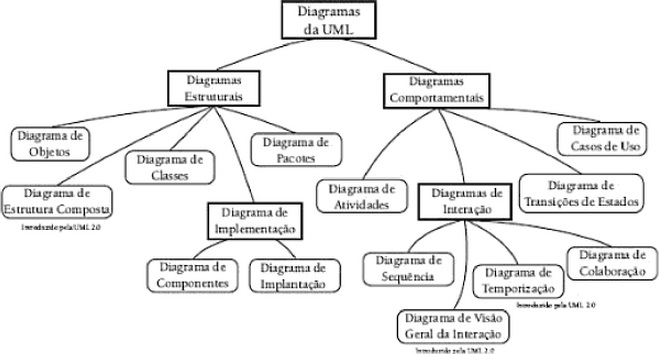
\includegraphics[scale=1]{./imagens/1_q_teorico/qt4.png}}
		\caption[Principais Diagramas definidos pela UML.]{Diagramas definidos pela
		UML. \textbf{Fonte:}\citeonline{2015principios}}
		\label{fig:qt4}
	\end{figure}
	\pagebreak
	
	\par A linguagem de modelagem UML não é processo rígido e permite uma
adequação de acordo com a situação do projeto em que é aplicada. Por permitir
essa flexibilidade e prover suporte adequado para determinados casos de um
projeto, será utilizada a linguagem de modelagem UML  para o desenvolvimento
desta pesquisa.